\documentclass{beamer}
\usepackage{luatexja}
\usepackage{graphicx}
\usepackage{hyperref}
\usepackage{listings,jvlisting}
\usepackage{luacode}
\usepackage{trig}

\usecolortheme[RGB={228,156,20}]{structure}
\usetheme{Madrid}

\newcommand\DegSin[1]{\CalculateSin{#1}\UseSin{#1}}
\newcommand\DegCos[1]{\CalculateCos{#1}\UseCos{#1}}
\newcommand\DegTan[1]{\CalculateTan{#1}\UseTan{#1}}

\setbeamertemplate{itemize item}[square]
\setbeamertemplate{itemize subitem}[circle]

\begin{luacode*}
    function to(i)
        j=i*math.pi/180
        return tostring(i).." & "..tostring(j).." & "..tostring(math.sin(j)).." & "..tostring(math.cos(j)).." & "..tostring(math.tan(j)).."\\\\"
    end
    
    function fg()
        v=""
        m="$\\vdots $ & $\\vdots $ & $\\vdots $ & $\\vdots $ & $\\vdots $ \\\\"
        for i=0,5,1 do
            v = v..to(i)
        end
        v=v..m
        for i=25,30,1 do
            v = v..to(i)
        end
        v=v..m
        for i=355,360,1 do
            v = v..to(i)
        end
        tex.sprint("\\newcommand{\\sd}{"..v.."}")
    end
\end{luacode*}
\directlua{ fg() }

\lstset{
  basicstyle=\tiny,
  frame={tb},
  breaklines=true,
  columns=[l]{fullflexible},
  numbers=left
}

\title{\LaTeX で作る三角関数表}
\author{椎木}

\begin{document}

\begin{frame}
    \titlepage
\end{frame}

\begin{frame}
\frametitle{レギュレーション解説}
\begin{itemize}
\setlength{\itemsep}{1cm}
\item 角度
\begin{itemize}
\item $0^\circ\rightarrow 5^\circ$
\item $25^\circ\rightarrow 30^\circ$
\item $355^\circ\rightarrow 360^\circ$
\end{itemize}
に対応するsin,cos,tanを表にまとめる.
\item 度数法は必ず記し,弧度法を使った場合は追記する.
\end{itemize}
\end{frame}

\begin{frame}
\frametitle{Excelでの手法}
\begin{columns}
    \begin{column}{0.49\textwidth}
        \begin{figure}
            \centering
            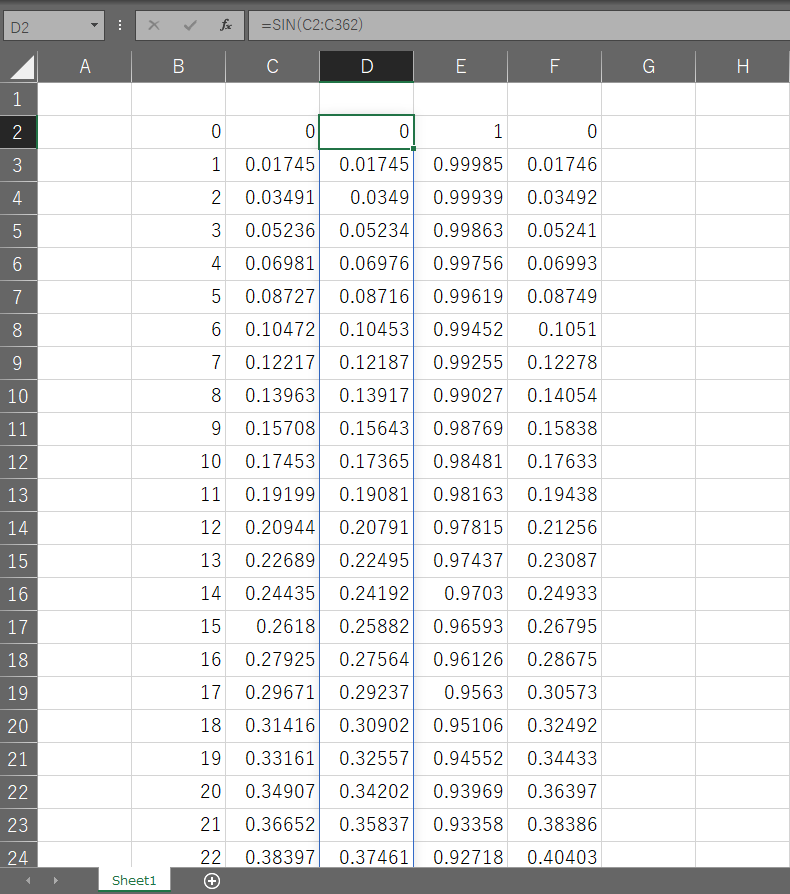
\includegraphics[scale=0.25]{ex.png}
        \end{figure}
    \end{column}
    \begin{column}{0.49\textwidth}
        \begin{table}[H]
            \centering
            \scalebox{0.5}{
            \begin{tabular}{cc|ccc}
                angle[$^\circ$]&angle[rad]&sin&cos&tan\\ \hline
                0 & 0 & 0 & 1 & 0 \\
                1 & 0.017453293 & 0.017452406 & 0.999847695 & 0.017455065 \\
                2 & 0.034906585 & 0.034899497 & 0.999390827 & 0.034920769 \\
                3 & 0.052359878 & 0.052335956 & 0.998629535 & 0.052407779 \\
                4 & 0.06981317 & 0.069756474 & 0.99756405 & 0.069926812 \\
                5 & 0.087266463 & 0.087155743 & 0.996194698 & 0.087488664 \\
                $\vdots $ & $\vdots $ & $\vdots $ & $\vdots $ & $\vdots $ \\
                25 & 0.436332313 & 0.422618262 & 0.906307787 & 0.466307658 \\
                26 & 0.453785606 & 0.438371147 & 0.898794046 & 0.487732589 \\
                27 & 0.471238898 & 0.4539905 & 0.891006524 & 0.509525449 \\
                28 & 0.488692191 & 0.469471563 & 0.882947593 & 0.531709432 \\
                29 & 0.506145483 & 0.48480962 & 0.874619707 & 0.554309051 \\
                30 & 0.523598776 & 0.5 & 0.866025404 & 0.577350269 \\
                $\vdots $ & $\vdots $ & $\vdots $ & $\vdots $ & $\vdots $ \\
                355 & 6.195918845 & -0.087155743 & 0.996194698 & -0.087488664 \\
                356 & 6.213372137 & -0.069756474 & 0.99756405 & -0.069926812 \\
                357 & 6.23082543 & -0.052335956 & 0.998629535 & -0.052407779 \\
                358 & 6.248278722 & -0.034899497 & 0.999390827 & -0.034920769 \\
                359 & 6.265732015 & -0.017452406 & 0.999847695 & -0.017455065 \\
                360 & 6.283185307 & -2.4503E-16 & 1 & -2.4503E-16 \\
                \\
            \end{tabular}
            }
        \end{table}
    \end{column}
\end{columns}
\vskip.3cm
\begin{itemize}
\item Excelで計算して\href{https://rra.yahansugi.com/scriptapplet/csv2tabular/}{csv2tabular}とかで変換するだけ.
\end{itemize}
\end{frame}

\begin{frame}[fragile]
\frametitle{trigでの手法}
\begin{columns}
    \begin{column}{0.49\textwidth}
\begin{lstlisting}
\usepackage{trig}
\newcommand\DegSin[1]{\CalculateSin{#1}\UseSin{#1}}
\newcommand\DegCos[1]{\CalculateCos{#1}\UseCos{#1}}
\newcommand\DegTan[1]{\CalculateTan{#1}\UseTan{#1}}
\begin{document}
\begin{table}[H]
  \centering
  \begin{tabular}{c|ccc}
    angle[$^\circ$]&sin&cos&tan\\ \hline
    0 & \DegSin{0} & \DegCos{0} & \DegTan{0} \\
  \end{tabular}
\end{table}
\end{lstlisting}
    \end{column}
    \begin{column}{0.49\textwidth}
        \begin{table}[H]
            \centering
            \scalebox{0.5}{
            \begin{tabular}{c|ccc}
                angle[$^\circ$]&sin&cos&tan\\ \hline
                0 & \DegSin{0} & \DegCos{0} & \DegTan{0} \\
                1 & \DegSin{1} & \DegCos{1} & \DegTan{1} \\
                2 & \DegSin{2} & \DegCos{2} & \DegTan{2} \\
                3 & \DegSin{3} & \DegCos{3} & \DegTan{3} \\
                4 & \DegSin{4} & \DegCos{4} & \DegTan{4} \\
                5 & \DegSin{5} & \DegCos{5} & \DegTan{5} \\
                $\vdots $ & $\vdots $ & $\vdots $ & $\vdots $ \\
                25 & \DegSin{25} & \DegCos{25} & \DegTan{25} \\
                26 & \DegSin{26} & \DegCos{26} & \DegTan{26} \\
                27 & \DegSin{27} & \DegCos{27} & \DegTan{27} \\
                28 & \DegSin{28} & \DegCos{28} & \DegTan{28} \\
                29 & \DegSin{29} & \DegCos{29} & \DegTan{29} \\
                30 & \DegSin{30} & \DegCos{30} & \DegTan{30} \\
                $\vdots $  & $\vdots $ & $\vdots $ & $\vdots $ \\
                355 & \DegSin{355} & \DegCos{355} & \DegTan{355} \\
                356 & \DegSin{356} & \DegCos{356} & \DegTan{356} \\
                357 & \DegSin{357} & \DegCos{357} & \DegTan{357} \\
                358 & \DegSin{358} & \DegCos{358} & \DegTan{358} \\
                359 & \DegSin{359} & \DegCos{359} & \DegTan{359} \\
                360 & \DegSin{360} & \DegCos{360} & \DegTan{360} \\
                \\
            \end{tabular}
            }
        \end{table}
    \end{column}
\end{columns}
\vskip.3cm
\begin{itemize}
\item trigによって\LaTeX 上で計算が出来る.
\end{itemize}
\end{frame}

\begin{frame}[fragile]
    \lstset{
  basicstyle=\fontsize{5.5pt}{0cm}\selectfont,
  frame={tb},
  breaklines=true,
  columns=[l]{fullflexible},
  numbers=left
}
    \frametitle{Luaでの手法}
    \begin{columns}
        \begin{column}{0.4\textwidth}
    \begin{lstlisting}
\usepackage{luacode}
\begin{luacode*}
  function to(i)
    j=i*math.pi/180
    return tostring(i).." & "..tostring(j).." & "..tostring(math.sin(j)).." & "..tostring(math.cos(j)).." & "..tostring(math.tan(j)).."\\\\"
  end
  function fg()
    v=""
    m="$\\vdots $ & $\\vdots $ & $\\vdots $ & $\\vdots $ & $\\vdots $ \\\\"
    for i=0,5,1 do
      v = v..to(i)
    end
    v=v..m
    for i=25,30,1 do
      v = v..to(i)
    end
    v=v..m
    for i=355,360,1 do
      v = v..to(i)
    end
    tex.sprint("\\newcommand{\\sd}{"..v.."}")
  end
\end{luacode*}
\directlua{ fg() }
\begin{document}
\begin{table}[H]
  \centering
  \caption{Lua言語を用いた三角関数表}
  \begin{tabular}{cc|ccc}
    angle[$^\circ$]&angle[rad]&sin&cos&tan\\ \hline
    \sd
    \\
  \end{tabular}
\end{table}
\end{document}
    \end{lstlisting}
        \end{column}
        \begin{column}{0.59\textwidth}
            \begin{table}[H]
                \centering
                \scalebox{0.4}{
                \begin{tabular}{cc|ccc}
                  angle[$^\circ$]&angle[rad]&sin&cos&tan\\ \hline
              \sd
              \\
              \end{tabular}
                }
              \end{table}
        \end{column}
    \end{columns}
    \begin{itemize}
    \item LuaによってLua\LaTeX 上で繰り返し計算及び表示が出来る.
    \end{itemize}
\end{frame}

\begin{frame}
    \frametitle{各手法の評価}
    \begin{table}[H]
        \centering
        \scalebox{1}{
        \begin{tabular}{rl|ll}
                & 手法  & 長所 & 短所 \\ \hline && \\
            2.1 & Excel & 簡単 & 
            \begin{tabular}{l}
                \LaTeX で完結しない \\ Excelに詳しい必要がある
            \end{tabular}\\ &&\\ 
            2.2 & trig  & \LaTeX で完結する & \begin{tabular}{l}
                文量が多い \\ 精度が良くない
            \end{tabular}\\ &&\\
            2.3 & Lua   & \begin{tabular}{l}
                Lua\LaTeX で完結する \\ きれいに書ける
            \end{tabular} & 難しい \\
      \\
      \end{tabular}
        }
      \end{table}
\end{frame}

\begin{frame}
    \frametitle{結論}
    \centering
    \Huge
    Excelで良いと思います
\end{frame}

\end{document}